% English IEEE conference research draft; all empirical claims refer to saved experiments.
\documentclass[conference,letterpaper,10pt]{IEEEtran}
\usepackage{amsmath,amssymb,bm,booktabs,array,graphicx}
\usepackage{cite}
\usepackage{balance}
\usepackage[hidelinks]{hyperref}
\hypersetup{pdftitle={Polynomial Nuisance Profiling for Range-Inertial Initialization},pdfauthor={Anonymous Authors},pdfsubject={IEEE conference research manuscript},pdfkeywords={UWB, inertial navigation, initialization, nuisance profiling, observability}}
\graphicspath{{recovery_bootstrap_figures/}}
\newtheorem{proposition}{Proposition}
\newtheorem{remark}{Remark}
\newcommand{\R}{\mathbb{R}}
\newcommand{\SO}{\mathrm{SO}}
\newcommand{\sk}[1]{[#1]_{\times}}
\newcommand{\norm}[1]{\left\lVert#1\right\rVert}
\newcommand{\rz}{R_z}
\newcommand{\ezz}{e_3}
\newcommand{\NormalProfileRMSE}{0.285}
\newcommand{\NormalProfileMax}{1.504}
\newcommand{\OutageProfileRMSE}{2.164}
\newcommand{\OutageProfileMax}{27.715}
\newcommand{\BiasFixedPosition}{0.737}
\newcommand{\BiasFreePosition}{0.073}
\newcommand{\BiasFixedYaw}{7.67}
\newcommand{\BiasFreeYaw}{0.92}

\title{Polynomial Nuisance Profiling for\\Range--Inertial Initialization}
\author{\IEEEauthorblockN{Anonymous Authors}
\IEEEauthorblockA{Working research manuscript --- 7 November 2026}}

\begin{document}
\maketitle

\begin{abstract}
Initializing range--inertial navigation far from surveyed anchors is sensitive to local minima and inertial calibration. We derive an initializer that separates yaw from unknown translation and polynomial inertial contamination. Squared asynchronous ranges yield a lift whose linear nuisance elimination leaves a quadratic objective on the unit circle, solved by quartic enumeration. We establish a sufficient noise-free recovery condition, polynomial-contamination invariance, and an explicit yaw--bias ambiguity. At 30 m stand-off with calibrated inertial displacement, profiling matches a twelve-start raw-range reference in all 200 excited-motion trials, compared with 159 for local initialization. The 95th-percentile position error decreases from $4.46$ to $0.51$ m and heading error from $155.5^\circ$ to $3.48^\circ$, with median desktop solve times of $11.9$ versus $59.9$ ms for twelve starts. Specified mild IMU calibration perturbations preserve the objective match in 200 further trials. Under a stronger combined perturbation, a quadratic nuisance model reduces the 95th-percentile position and heading errors from $4.54$ m and $54.85^\circ$ to $0.76$ m and $12.39^\circ$ against an affine model with the same two-seed policy, at a cost in ideal-input accuracy. Across 528 paired real-data window configurations, one profiled candidate reduces misses of the best observed raw objective from 87 to 40. Weak vertical geometry, unobservable yaw--bias combinations, and complete-filter outage transients delimit the demonstrated benefit.
\end{abstract}

\begin{IEEEkeywords}
Ultra-wideband localization, inertial navigation, invariant extended Kalman filter, initialization, observability, robust estimation.
\end{IEEEkeywords}

\section{Introduction}
Two-way ranging (TWR) measures distance between an ultra-wideband (UWB) tag and a surveyed anchor. When initial position or heading is unreliable, a local filter must interpret spherical observations at an uncertain linearization point while propagating body-frame inertial measurements. Accepting a range update does not establish that all navigation states are observable or that reliable tracking has begun.

Invariant filtering is relevant to this problem because it structures navigation errors on a Lie group. Oursland and Mehrabian studied IMU--UWB fusion with particular attention to large heading errors\cite{oursland2024}. Their measurement model uses time differences of arrival and a tag lever arm. The present study retains invariant inertial tracking but considers a different acquisition problem: a single tag, known anchors, asynchronous TWR, and a zero lever arm. The two settings cannot be ranked directly through their published numerical results. Likewise, local stability results for appropriate invariant observers\cite{barrau2017} do not provide an automatic global-convergence guarantee for an arbitrary biased, gated, range-aided implementation.

Two difficulties motivate this work. A wide prior can accommodate a large initialization error but also permit a corrupted measurement to cause a large excursion; early rejection can instead prevent acquisition. Moreover, a short window can fit ranges while inferring heading through an assumed accelerometer calibration. A direction well constrained under fixed bias can become unobservable when bias is uncertain.

We investigate candidate generation before a complete acquisition supervisor. An inertial displacement, known up to vertical rotation, is combined with a translation polynomial. Range expansion eliminates linear nuisance variables and leaves two circular coordinates, supplying yaw candidates without an initial position or heading guess. Auxiliary norm and cross-product variables are temporarily independent; original ranges provide the final refinement.

This work provides three results. First, an explicit yaw-profile construction specialized to inertial displacement yields a finite candidate enumeration and a sufficient noise-free recovery condition. Second, polynomial-contamination invariance explains exactly which inertial errors translation can absorb, while an ambiguity construction and a bounded-rotation approximation delimit that protection. Third, paired geometry stress tests demonstrate a larger practical acquisition basin than a single raw-range refinement, approaching the twelve-start reference at substantially lower measured cost. Window-level real measurements and complete invariant-filter replays separate initialization reliability from eventual tracking accuracy. Generic squared-range lifting, polynomial solvers, and information projection are established techniques; the contribution is their specialization to inertial shape and bias-related nuisance directions, with explicit conditions and matched baselines.

\section{Related Work and Scope}
Pacholska, D\"umbgen, and Scholefield recover continuous trajectories from asynchronous distances to known anchors using polynomial or bandlimited bases and linear relaxation\cite{pacholska2020}. This close antecedent already establishes polynomial range lifting and recovery conditions. Our specialization separates an inertially supplied displacement from its unknown yaw, reduces the rotational constraint to a circle, and evaluates its benefit against robust initialization baselines.

Goudar \emph{et al.} develop semidefinite relaxations for static and constant-velocity range-only initialization\cite{goudar2024}. Trawny and Roumeliotis solve planar relative pose from ranges and known egomotion algebraically\cite{trawny2010}; Molina Martel \emph{et al.} initialize four-degree-of-freedom pose from ranges and visual-SLAM trajectories\cite{molina2019}. Our model additionally profiles unknown velocity and bias-related translation. An adapted semidefinite benchmark remains missing.

Ge \emph{et al.} study equivariant range-only SLAM\cite{ge2025}, and Fornasier \emph{et al.} analyze inertial-navigation symmetries and bias treatment\cite{fornasier2025}. Unknown-landmark SLAM and known-anchor initialization have different gauge structures. Motion- and bias-dependent observability is also established\cite{hong2005}; our counterexample specializes this issue to the proposed window model.

Pfeiffer \emph{et al.} develop efficient UWB moving-horizon estimation\cite{pfeiffer2021} and subsequently improve step sizes and outlier handling\cite{pfeiffer2025}. Their public data supply our real measurements\cite{pfeifferdata2021}. The 2025 estimator is not reproduced here, limiting state-of-the-art claims; our comparison isolates initialization and re-entry into a common invariant tracker.

Jiang \emph{et al.} combine single-sided TWR and IMU data using an asymmetric half-Cauchy ranging model, a ten-second joint factor-graph initialization, and damped incremental smoothing\cite{jiang2024}. Their complete system is a strong additional benchmark not reproduced here; our contribution is a specialized algebraic yaw candidate and polynomial nuisance analysis, rather than a claim to originate robust ranging--IMU acquisition.

\section{Problem Formulation}
Let $a_i\in\R^3$ be a surveyed anchor and let the bias-corrected range at its actual transaction time be
\begin{equation}
 r_i=z_i-\beta_i=\rho_i+e_i,\qquad
 \rho_i=\norm{p(t_i)-a_i}.
 \label{eq:range}
\end{equation}
The tag lever arm is zero. Independent Gaussian $e_i\sim\mathcal N(0,\sigma_i^2)$ is used only for the inlier noise calculation; contaminated and real measurements need not follow that model. The anchor bias $\beta_i$ and scale $\sigma_i$ are fixed before an evaluation replay.

The nominal inertial model is
\begin{align}
 \dot R&=R\sk{\omega_m-b_g}, & \dot p&=v,\nonumber\\
 \dot v&=R(f_m-b_a)+g, & g&=-g_0 e_3,
 \label{eq:ins}
\end{align}
with $g_0=9.81\,\mathrm{m/s^2}$. Static acceleration constrains the gravity direction but does not determine yaw. Over a short window, first assume known biases and write $R(t)=\rz(\psi)Q(t)$, where $Q$ is propagated from gravity alignment with the measured gyroscope. With the final window time $T$ as reference and $\tau=t-T$, reanchor the integrated displacement so that $d(T)=\dot d(T)=0$. Since a vertical rotation leaves gravity unchanged,
\begin{equation}
 p(t)=p_T+v_T\tau+\rz(\psi)d(t).
 \label{eq:affine}
\end{equation}
This identity is exact for the corresponding discrete, held-sample inertial model when the biases and initial tilt are correct. It is not exact for arbitrary bias errors.

For the algebra and a restricted bias extension, use
\begin{equation}
 p(t)=c(t)+\rz(\psi)d(t),\qquad
 c(t)=\sum_{j=0}^{K}c_j\tau^j.
 \label{eq:poly}
\end{equation}
The primary initializer uses $K=1$. Under constant attitude, a constant body accelerometer-bias error produces a constant world acceleration error and is absorbed by $K=2$. This extension is exact only under that condition. With varying attitude, the correct sensitivity is a double integral of $Q(t)$, rather than a scalar quadratic term; the corresponding model is discussed in Section~\ref{sec:limits}.

\section{A Profiled Yaw Candidate}
\subsection{Exact Lift of the Squared Range}
Temporarily consider noise-free ranges. Define
\begin{equation}
 y_i=\tfrac12\bigl(r_i^2-\norm{a_i}^2-\norm{d_i}^2\bigr)+a_{iz}d_{iz}.
 \label{eq:y}
\end{equation}
Expanding \eqref{eq:range}--\eqref{eq:poly} yields
\begin{equation}
 y=B\nu+D c+C u,\qquad
 u=\begin{bmatrix}\cos\psi&\sin\psi\end{bmatrix}^{\!\top}.
 \label{eq:lift}
\end{equation}
Here $c$ stacks the $K+1$ three-vectors $c_j$. The row blocks are
\begin{align}
 B_i&=\left[\{\tau_i^\ell\}_{\ell=0}^{2K},
       \{\tau_i^j d_{ix},\tau_i^j d_{iy}\}_{j=0}^{K}\right],\label{eq:b}\\
 D_{ij}&=\tau_i^j\begin{bmatrix}-a_{ix}&-a_{iy}&d_{iz}-a_{iz}\end{bmatrix},\label{eq:d}\\
 C_i&=\begin{bmatrix}
  -a_{ix}d_{ix}-a_{iy}d_{iy}&a_{ix}d_{iy}-a_{iy}d_{ix}
 \end{bmatrix}.\label{eq:c}
\end{align}
The first $2K+1$ components of $\nu$ are the coefficients of $\frac12\norm{c(t)}^2$. Its remaining components are the horizontal entries of $\rz(\psi)^\top c_j$. The vertical cross terms are retained in $D$ because a yaw rotation leaves $c_{jz}$ unchanged. Thus $\nu$ has $4K+3$ components, and $[\nu^\top,c^\top]^\top$ has $7K+6$. For $K=1$ and $K=2$, the complete lifts contain 15 and 22 scalar coordinates, respectively, including the two entries of $u$.

Equation~\eqref{eq:lift} is an exact algebraic identity on the physical parameter set. Treating $\nu$ as independent of $c$ and $u$ enlarges that set. This distinction matters: a minimizer of the relaxed squared-range problem need not minimize the physically constrained raw-range problem.

\subsection{Eliminating Linear Nuisances}
Let $W$ be a positive diagonal whitening matrix and define
\begin{equation}
 \begin{aligned}
 L&=W[B\ D],& P_L&=I-LL^{\dagger},\\
 \bar y&=P_LWy,& \bar C&=P_LWC.
 \end{aligned}
 \label{eq:projection}
\end{equation}
The projector is applied through a rank-revealing singular value decomposition; no dense $N\times N$ projector is stored. Eliminating the linear variables gives
\begin{equation}
 \min_{\norm{u}=1}\norm{\bar y-\bar C u}^2
 =\min_{\norm{u}=1}u^\top H u-2h^\top u+\mathrm{const},
 \label{eq:circle}
\end{equation}
where $H=\bar C^\top\bar C$ and $h=\bar C^\top\bar y$. The model dimension is fixed for a chosen $K$; increasing the number of transactions adds rows rather than optimization states.

Set $\Delta=H_{22}-H_{11}$ and $q=\tan(\psi/2)$. The stationary-angle equation becomes
\begin{align}
 0={}&(H_{12}+h_2)q^4+2(h_1-\Delta)q^3-6H_{12}q^2\nonumber\\
    &+2(h_1+\Delta)q+(H_{12}-h_2).
 \label{eq:quartic}
\end{align}
We enumerate the real roots, map them back to the circle, include $\psi=\pi$ to cover the point omitted by the half-angle chart, and evaluate \eqref{eq:circle}. Degenerate constant objectives are handled directly. This enumeration finds the global minimum of the two-dimensional relaxed problem. It does not establish global optimality of a subsequent nonlinear raw-range refinement.

\begin{proposition}[Sufficient exact yaw recovery]
Assume noiseless ranges generated by \eqref{eq:poly}, an exact inertial displacement, and a positive diagonal $W$. If $\operatorname{rank}(\bar C)=2$, the global minimizer of \eqref{eq:circle} is the true $u$, and hence the true yaw modulo $2\pi$. Given that yaw, translation is unique if
\begin{equation}
 \operatorname{rank}\!\left(P_{WB}WD\right)=3(K+1),\qquad
 P_{WB}=I-(WB)(WB)^{\dagger}.
 \label{eq:translationrank}
\end{equation}
\end{proposition}
\begin{IEEEproof}
The true physical variables satisfy \eqref{eq:lift}, so their projected residual is zero. Any global minimizer therefore satisfies $\bar C(u-u_\star)=0$. Full column rank implies $u=u_\star$. With $u$ fixed, eliminating $\nu$ leaves a linear system in $c$ whose coefficient matrix is $P_{WB}WD$; \eqref{eq:translationrank} implies a unique solution.
\end{IEEEproof}

These conditions are sufficient, not necessary. A rank-deficient relaxation can discard information still present in the nonlinear consistency relations among the lifted variables. It cannot, on that basis alone, certify that the original physical model is unobservable. Conversely, full rank in ideal data is not an error bound under calibration errors or contaminated ranges.

\subsection{Noise Treatment and Raw-Range Refinement}
For Gaussian inlier noise in \eqref{eq:range}, replace $r_i^2$ in \eqref{eq:y} by $r_i^2-\sigma_i^2$. The remaining random part is
\begin{equation}
 \epsilon_i=\rho_i e_i+\tfrac12(e_i^2-\sigma_i^2),\quad
 \mathbb E[\epsilon_i]=0,\quad
 \operatorname{var}(\epsilon_i)=\rho_i^2\sigma_i^2+\tfrac12\sigma_i^4.
 \label{eq:squarednoise}
\end{equation}
The true $\rho_i$ is unavailable. The implementation uses a positive plug-in scale based on the observed corrected range; this introduces random weights and is an approximation. Squared residuals are non-Gaussian, and inertial preintegration error couples transactions. Neither effect is eliminated by the algebraic projection.

Accordingly, the lift supplies a yaw candidate, after which we minimize
\begin{equation}
 J(c,\psi)=\sum_i\rho_H\!\left(
 \frac{\norm{c(t_i)+\rz(\psi)d_i-a_i}-r_i}{\sigma_i}\right),
 \label{eq:rawcost}
\end{equation}
where $\rho_H$ is the Huber loss with normalized threshold 2. For $K=1$, robust constant-velocity localization supplies the translation seed, because recovering translation from the relaxed lift can be ill conditioned. The exact-recovery proposition concerns the lifted candidate primitive; it does not transfer automatically to this CV-seeded nonlinear pipeline. The analytic Jacobian includes
\begin{equation}
 J_{c_j,i}=\frac{\tau_i^j n_i^\top}{\sigma_i},\qquad
 J_{\psi,i}=\frac{n_i^\top\sk{e_3}\rz(\psi)d_i}{\sigma_i},
 \label{eq:jacobian}
\end{equation}
where $n_i=(p(t_i)-a_i)/\norm{p(t_i)-a_i}$ is the unit range direction. The optimizer is capped at 120 function evaluations. A twelve-start reference uses uniformly spaced yaw seeds and the same raw cost, translation seed, stopping rules, and range scales.

\section{Bias, Identifiability, and Handoff}
\subsection{Why a Fixed-Bias Yaw Test Can Be Misleading}
Partition a weighted raw-range Jacobian into nuisance and yaw columns, $A=[A_n\ a_\psi]$. A local information measure after nuisance elimination is
\begin{equation}
 \mathcal I_{\psi\mid n}=\norm{(I-A_nA_n^{\dagger})a_\psi}^2.
 \label{eq:information}
\end{equation}
The result has units of inverse squared radians. In robust estimation, $A=\operatorname{diag}(\sqrt{w_i})J$ uses final Huber iteratively reweighted least-squares (IRLS) weights. Thus $A^\top A$ is an IRLS surrogate information matrix, not the exact Hessian of the Huber objective or a validated posterior precision. The choice of nuisance columns is essential. Eliminating only $p_T,v_T$ measures heading information conditional on fixed biases. Including bias-sensitive columns answers a different question.

\begin{proposition}[Constant-acceleration ambiguity]
Suppose attitude is constant, the gyroscope bias is known, and the measured specific force $f_m$ is constant over a window. If the constant accelerometer bias is unrestricted, position-only ranges cannot identify yaw, even with nondegenerate surveyed anchors and noiseless, arbitrarily frequent measurements.
\end{proposition}
\begin{IEEEproof}
Let a solution have $R=\rz(\psi)Q$ and bias $b_a$. For any candidate yaw $\psi'$, define
\begin{equation}
 b_a'=f_m-Q^\top\rz(\psi')^\top\rz(\psi)Q(f_m-b_a).
 \label{eq:biasambiguity}
\end{equation}
Because $Q$ and $f_m$ are constant, $b_a'$ is constant. Substitution gives $\rz(\psi')Q(f_m-b_a')=\rz(\psi)Q(f_m-b_a)$. The acceleration, and therefore the entire position trajectory with the same initial position and velocity, is unchanged. All zero-lever-arm ranges are identical for this continuum of yaw--bias pairs.
\end{IEEEproof}

For the quadratic translation model, the same effect appears in \eqref{eq:information}: the yaw sensitivity of a quadratic inertial displacement lies in the span of the quadratic translation columns. Its projected information is zero. With varying acceleration, the nonquadratic component can retain heading information after constant-bias elimination. This does not imply that any small amount of variation is practically sufficient: the informative component must remain distinguishable from noise, calibration uncertainty, and model mismatch.

\begin{proposition}[Polynomial nuisance invariance]
Let all translation coefficients in \eqref{eq:poly} be unrestricted. Replacing $d(t)$ by $d'(t)=d(t)+b(t)$, where $b(t)=\sum_{j=0}^{K}b_j\tau^j$, leaves the raw-range objective profiled over translation unchanged for every yaw. It also leaves the nuisance-projected local yaw information unchanged at corresponding states. The relaxed circle objective is unchanged when $W$ depends only on the unchanged ranges and their scales.
\end{proposition}
\begin{IEEEproof}
For every $\psi$, set $c_j'=c_j-\rz(\psi)b_j$. Then $c'(t)+\rz(\psi)d'(t)=c(t)+\rz(\psi)d(t)$, so corresponding residuals and any residual-based robust weights are identical. The change in the yaw Jacobian is a linear combination of the translation columns and is removed in \eqref{eq:information}. For the lift, the column space of $B$ is unchanged because $\tau^j b_x$ and $\tau^j b_y$ have degree at most $2K$. Changes in $D$ lie in that space; changes in $C$ lie in the space of $[B\ D]$; and the change in $y$ is a combination of the same polynomial and cross-term columns. Projection therefore leaves $\bar y$ and $\bar C$ unchanged.
\end{IEEEproof}

This invariance explains why the free-bias synthetic results are nearly identical across bias magnitudes for a fixed seed. They are repeated perturbations of the same equivalence class, not three independent demonstrations of general bias robustness. Constant world acceleration bias is a quadratic contamination; arbitrary rotating-body bias or gyroscope bias is not.

\begin{proposition}[Bounded-rotation approximation]
Let $Q$ be absolutely continuous on $[t,T]$ with $\norm{\dot Q(s)}_2\le\Omega$ almost everywhere, and define the endpoint-reanchored bias sensitivity
\begin{equation}
 B_e(t)=\int_t^T(s-t)Q(s)\,ds.
\end{equation}
Then
\begin{equation}
 \norm{B_e(t)-\tfrac12(T-t)^2Q(T)}_2
 \le\frac{\Omega}{6}(T-t)^3.
 \label{eq:rotationbound}
\end{equation}
Consequently, a constant body-bias perturbation $\delta b_a$ is absorbed by the $K=2$ model up to a displacement remainder, and hence a raw-range perturbation, bounded by $\Omega\norm{\delta b_a}|t-T|^3/6$.
\end{proposition}
\begin{IEEEproof}
Absolute continuity gives $\norm{Q(s)-Q(T)}_2\le\Omega(T-s)$. Integrating $(s-t)\Omega(T-s)$ from $t$ to $T$ gives \eqref{eq:rotationbound}. Multiplication by $\delta b_a$ and a yaw rotation preserves the bound, and the reverse triangle inequality bounds the resulting range change.
\end{IEEEproof}
This deterministic approximation quantifies the interaction of rotation rate, bias magnitude, and window duration. It does not bound the estimation error after an ill-conditioned inverse problem or account for gyroscope-bias uncertainty.

An isolated initial tilt error has a related structure. With exact subsequent gyroscope increments and specific force, $\hat Q(t)=E Q(t)$ for constant $E$, giving $\hat d(t)=E d(t)+\tfrac12\tau^2(I-E)g$. Quadratic translation absorbs the gravity term exactly; the remaining shape error is bounded by $2\sin(\theta_E/2)\norm{d(t)}$, where $\theta_E$ is the rotation angle of $E$. Gyroscope errors generally make $E$ time varying, so this identity does not establish combined-error invariance.

\begin{figure}[t]
 \centering
 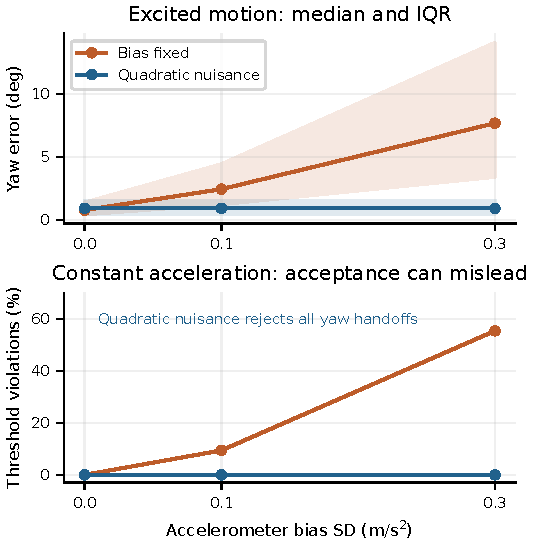
\includegraphics[width=\columnwidth]{bias_tradeoff.pdf}
 \caption{Controlled bias study. Fixed-bias information can remain large while heading and position errors increase. The quadratic nuisance model removes constant-acceleration heading information; under excited motion it can estimate the added bias contribution. Rejected heading estimates represent unavailable heading information, not successful heading recovery.}
 \label{fig:bias}
\end{figure}

\subsection{Causal Acquisition and a Common Invariant Tracker}
A cold start consumes 1.5 s of IMU data for gravity alignment and static bias estimation. The fixed-window initializers then collect 2 s of changed, positive TWR transactions. No runtime position truth is passed to the estimator. During a ranging outage, the active tracker continues propagation. When a new transaction follows a measured inter-arrival gap greater than 1 s, a new capture window starts. The trigger uses actual transaction arrival times, not knowledge of the scripted outage endpoint.

At an accepted window endpoint, the estimated position, velocity, yaw, and their joint local uncertainty initialize a single 15-state invariant tracker. Its error ordering is $[\theta,v,p,b_g,b_a]$. Let $P_e$ describe body-right attitude and additive world velocity and position errors. For state $X=(R,v,p)$, the invariant chart map is
\begin{equation}
 C_X=\begin{bmatrix}
 R&0&0&0&0\\
 \sk{v}R&I&0&0&0\\
 \sk{p}R&0&I&0&0\\
 0&0&0&I&0\\0&0&0&0&I
 \end{bmatrix},\qquad P_r=C_XP_eC_X^\top.
 \label{eq:chart}
\end{equation}
The endpoint yaw increment maps to the body attitude direction $R^\top e_3$. The implementation retains the estimated position--velocity--yaw cross terms and adds explicit uncertainty for tilt, biases, and model mismatch. Broad finite priors regularize unobserved directions; they must not be mistaken for information from ranges. In particular, a pseudoinverse of a singular information matrix would assign zero variance to its nullspace and is unsuitable as a standalone covariance.

The tracker uses the common held-sample inertial model and the complete range Jacobian under left group injection, corresponding to the right-invariant error $X_{\mathrm{true}}\hat X^{-1}$:
\begin{equation}
 H_r=\begin{bmatrix}-n^\top\sk{p}&0&n^\top&0&0\end{bmatrix}.
 \label{eq:hr}
\end{equation}
The physical-to-invariant covariance conversion and reset are applied consistently. Range updates use a normalized innovation gate of $12.25$ and a Huber threshold of 2. Newly initialized trackers apply this policy immediately. The empirical covariance floors are $0.15$ m for position, $0.20$ m/s for velocity, and $0.10$ rad for yaw; they are not calibrated coverage guarantees.

All capture measurements are consumed at the handoff endpoint. The new tracker processes only subsequent events, preventing explicit replay of the same ranges as independent new measurements. This data-use rule is necessary but not sufficient for full statistical consistency: inertial integration, calibration, and any reused nuisance priors introduce correlations that this prototype does not fully propagate.

\subsection{A Deliberately Simple Information-Triggered Ablation}
An adaptive variant attempts 2, 4, and 8 s windows. It accepts when the fixed-bias measure satisfies $\mathcal I_{\psi\mid p,v}\ge1/(0.35\,\mathrm{rad})^2$ and the normalized residual RMS is at most 3. These are provisional engineering thresholds. The bias counterexample explains why they are not a certificate. If no attempt qualifies, the absence of an initialized output is retained in the result. A low error conditional on producing output must be reported alongside availability and acquisition delay.

\section{Experimental Protocol}
\subsection{Synthetic Studies}
The first study uses eight anchors at $(\pm4,\pm4,0)$ and $(\pm4,\pm4,3)$ m, 240 asynchronous transactions over a four-second interval, uniformly random initial yaw, and $0.10$ m Gaussian range noise. It compares constant-velocity, local inertial, twelve-start inertial, and profiled inertial initialization for constant velocity, constant acceleration, and excited motion. A second noise condition adds $1.5$ m to a random 5\% of transactions. Two hundred seeds per condition give 4,800 estimator trials. Identical seeds pair methods on the same data. The supplied inertial displacement is exact in this study, so the result isolates initialization geometry rather than a complete noisy IMU pipeline.

The bias study adds a constant vector with component standard deviation $0$, $0.1$, or $0.3\,\mathrm{m/s^2}$ to the integrated acceleration. Fixed-bias $K=1$ estimation is compared with the $K=2$ free-bias polynomial model under excited and constant-acceleration motion. One thousand paired seeds per motion and magnitude give 12,000 estimator trials. The two methods share ranges, geometry, and perturbations. Reported position is the polynomial coefficient at the reference time; heading is compared modulo $2\pi$. An ``accepted but inaccurate'' heading is one satisfying the provisional information threshold while its absolute error exceeds $0.35$ rad. This event is not a failure of a nominal 95\% confidence interval, because no such interval has been calibrated.

\subsection{Stand-Off and Vertical-Geometry Stress Test}\label{sec:geometryprotocol}
To probe a larger acquisition region, a separate study places the reference endpoint at horizontal radius $r\in\{10,30\}$ m from the anchor centroid, uniformly random azimuth, and height 1.2 m. The eight anchors are $(\pm4,\pm4,z)$ m with $z\in\{0,h\}$ and vertical span $h\in\{0.1,3\}$ m. Yaw is independently uniform over $[-\pi,\pi)$, and each velocity component is uniform over $[-0.5,0.5]$ m/s. There are 240 asynchronous transactions at sorted random times in $[-4,0]$ s, with independently selected anchors and $0.10$ m Gaussian range noise. The displacement is exact and biases are calibrated, isolating geometry and optimization.

The two endpoint-reanchored inertial shapes are
\begin{align}
 d_{\rm exc}(\tau)&=\begin{bmatrix}
 0.8\sin(1.7\tau)-1.36\tau\\
 0.6\bigl(\cos(1.1\tau)-1\bigr)\\
 0.15\sin(0.7\tau)-0.105\tau
 \end{bmatrix},\label{eq:excitedshape}\\
 d_{\rm acc}(\tau)&=\tfrac12\tau^2
 \begin{bmatrix}0.4&-0.3&0.1\end{bmatrix}^{\!\top}.
\end{align}
Both satisfy $d(0)=\dot d(0)=0$. Two hundred new seeds in each of the eight geometry--motion cells are paired across four methods, giving 6,400 fits. A raw-range objective miss means
\begin{equation}
 J-J_{12}>\max\{10^{-3},10^{-5}|J_{12}|\},
 \label{eq:objectivegap}
\end{equation}
where $J_{12}$ is the twelve-start objective on the identical data. This is a comparison with a strong finite reference, not a global-optimality certificate or a truth-error threshold. CV uses a different motion model and is excluded from this optimization-miss comparison.

\subsection{Inertial Calibration Mismatch}\label{sec:imuprotocol}
A further simulation retains the 30 m stand-off, 3 m anchor-height span, excited acceleration, and range-noise model, but generates physical specific-force and angular-rate samples at 200 Hz. The true yaw-free attitude is
\begin{equation}
 Q(t)=R_y\!\left(8^\circ\sin(1.3t)\right)
       R_x\!\left(10^\circ\sin(0.9t)\right),\quad t\in[0,4].
\end{equation}
For acceleration $a_k$ in this gravity-aligned frame, the specific force is $Q_k^\top(a_k-g)$ and angular rate is $\log(Q_k^\top Q_{k+1})^\vee/\Delta t$, with $\Delta t=0.005$ s. True world acceleration is $\rz(\psi)a_k$. The measured shape is propagated with constant accelerometer and gyroscope bias errors and a body-right initial tilt perturbation $\exp([\delta\theta_x,\delta\theta_y,0]_\times)$, using the same held-sample integration and endpoint reanchoring as truth.

The ideal, mild, and moderate levels use component standard deviations $(\sigma_a,\sigma_g,\sigma_{\theta})$ of $(0,0,0)$, $(0.02,0.002,0.5^\circ)$, and $(0.10,0.01,2^\circ)$, respectively, with acceleration in $\mathrm{m/s^2}$ and angular rate in rad/s. Two hundred new seeds share ranges and standardized perturbation draws across three levels and three $K=1$ methods, giving 1,800 fits. There is no IMU measurement white noise. This is a combined calibration-mismatch stress test, not an isolated causal ablation of each error source. Heading error is computed from the physical endpoint orientation $\rz(\hat\psi)\hat Q(T)$, rather than only the scalar yaw parameter. Objective misses use \eqref{eq:objectivegap}.

A matched model-order ablation adds 1,200 fits on these same 600 seed--level combinations. Both $K=1$ and $K=2$ use two translation seeds: their recovered lifted translation and a common CV translation, with zero quadratic coefficient when needed. Both seeds use the respective lifted yaw and identical robust refinement rules. This compares model order and its induced lift under the same seed policy; it differs from the main one-refinement profile pipeline. Objectives are not ranked across different motion models.

\subsection{Real TWR Replays}
We use twelve logs from the public TU Delft data\cite{pfeifferdata2021}: two each for triangle, octagon, hourglass, random, star, and square motion. All were collected on the same date. The chronologically earlier log of each motion supplies calibration; the later log is evaluated. The evaluation recordings last approximately 38--64 s after the IMU prefix. Each anchor's range bias is a training-residual median, and its scale is $1.4826$ times the median absolute deviation, clipped to $[0.08,0.50]$ m. Both IMU and UWB timestamps receive the existing common $0.20$ s alignment correction relative to OptiTrack. This is offline evaluation alignment, not an online relative IMU--UWB delay estimate.

Changed-range detection follows the logger's held-value semantics. Zero ranges are missing transactions. The estimator uses known anchor coordinates, IMU data, and these range events. Ground truth is used for calibration on the separate six logs, selecting a valid evaluation interval, and offline scoring; it does not initialize position at runtime. All twelve logs have been exposed during prior project development, so this split isolates calibration within the present experiment but is not independent blind testing.

Eight methods are evaluated on six logs, with and without suppression of ranges during $[15,25)$ s, giving 96 complete replays. Besides the four window methods and the adaptive variant, controls include an invariant tracker initialized at the anchor centroid, a two-second lifted capture followed by that tracker, and the same lifted capture with gating active from the first update. The historical lifted controls retain their own acquisition covariance and warm-up settings; they therefore compare complete acquisition policies, not an isolated change of yaw seeding. Their ordinary configuration suppresses both hard rejection and Huber weighting for the first 256 valid updates.

Stable success means that the position error stays at or below $0.5$ m for the complete remaining recording, with at least 5 s observed after the final threshold crossing. Outage recovery is timed from 25 s. An unsuccessful record can reflect a late excursion or insufficient remaining observation, rather than permanent mathematical divergence. We retain finite but very large errors. No numerical failure is discarded.

The common position-RMSE interval starts at 8.1 s, after the largest candidate startup window. We additionally report output availability, initial unavailable time, terminal five-second RMSE, and the maximum over all available outputs. Window initializers have no output before their first handoff; this latency is not silently replaced by ground truth or a retrospectively smoothed trajectory. During recapture, an existing tracker's propagated output remains visible and contributes its error.

\subsection{Matched Real-Window Candidate Comparison}\label{sec:realwindowprotocol}
To isolate initialization from the subsequent tracker, we extract eleven windows from each of the six evaluation recordings: durations 2 and 4 s ending at 5 s, and durations 2, 4, and 8 s ending at 10, 20, and 30 s. We use both all eight anchors and the transactions from the four anchors with lowest surveyed height. Each window is expressed in four inertial yaw frames, $\phi\in\{0,\pi/2,\pi,3\pi/2\}$, by replacing $d$ with $\rz(\phi)d$ and the physical yaw coordinate with $\psi-\phi$. This leaves the trajectory family and optimum unchanged; the common CV position and velocity seed is unchanged. These 528 configurations are paired computational stress cases from 66 physical windows, not 528 independent recordings.

Six methods minimize the same robust raw-range objective: one local yaw seed; the lowest-cost relaxed-circle seed (Profile-1); the two lowest-cost distinct circle candidates (Profile-2); all real stationary candidates plus auxiliary $0$ and $\pi$ seeds (Profile-all); four uniformly spaced yaw seeds (Uniform-4); and twelve uniformly spaced seeds (Uniform-12). Circular duplicates within $10^{-7}$ rad are removed. Profile-all uses a median of four seeds and at most six. A miss exceeds the best objective observed among all six methods by $10^{-4}(1+J_{\rm best})$. No ground-truth position is used to initialize or rank candidates. Counts are also checked at relative tolerances $10^{-3}$ and $10^{-2}$. Function-evaluation totals include both least-squares solves used to construct the common CV seed as well as all raw-range refinements.

\begin{table*}[t]
\caption{Real-data development replays: six logs per regime. RMSE is the median across logs on the common $t\ge8.1$ s interval; maximum is over all available outputs and all six logs. Availability is reported separately.}
\label{tab:real}
\centering
\setlength{\tabcolsep}{5.3pt}
\begin{tabular}{lrrrrrrr}
\toprule
&\multicolumn{4}{c}{Continuous ranging}&\multicolumn{3}{c}{Ten-second outage}\\
\cmidrule(lr){2-5}\cmidrule(lr){6-8}
Method&Success&RMSE (m)&Max. (m)&Startup delay (s)&Success&RMSE (m)&Max. (m)\\
\midrule
Centroid InEKF&4/6&0.302&20835.647&0&4/6&7.923&20835.647\\
Lifted capture&5/6&0.285&16.265&0&5/6&1.387&17.648\\
Lifted, gate from start&4/6&0.285&2181.290&0&4/6&1.815&6118.259\\
Robust CV window&5/6&0.285&1.504&2&5/6&2.349&25.863\\
Local inertial window&5/6&0.285&1.504&2&5/6&2.164&27.715\\
Twelve-start inertial&5/6&0.285&1.504&2&5/6&2.164&27.715\\
Profiled inertial&5/6&\NormalProfileRMSE&\NormalProfileMax&2&5/6&\OutageProfileRMSE&\OutageProfileMax\\
Adaptive profile&4/6&0.283$^{\dagger}$&1.536&4$^{\ddagger}$&5/6&2.249$^{\dagger}$&22.623\\
\bottomrule
\end{tabular}
\par\vspace{3pt}\footnotesize
$^{\dagger}$Adaptive common-interval availability is 83.3\% with continuous ranging and 94.4\% with an outage; its conditional RMSE is not directly comparable to a fully available estimator.
$^{\ddagger}$Median across logs; one continuous-ranging log never initializes. All other methods have 100\% common-interval availability.
\end{table*}

\section{Results}
\subsection{Algebraic Verification and Near-Field Controls}
The verification suite checks the exact lift against independently generated noise-free positions, all analytic raw-range derivatives against central finite differences, the circular solver against a dense independent angular grid, and the bias-induced yaw nullspace. The generalized quadratic lift is tested separately. These checks validate the algebra and its implementation; they do not establish real-data generalization or a new global observer theorem.

In the original excited synthetic motion without added bias, the profiled, local, and twelve-start inertial methods reach effectively the same raw-range objective and median position and yaw errors. Their median position error is $0.048$ m under Gaussian noise and $0.058$ m with contamination. These near-field controls verify matched accuracy in an easier regime. Constant-velocity ranges can still recover position while yaw remains unconstrained.

A limited tail benefit appears under constant acceleration: in each noise setting, one of 200 local refinements has an objective more than $10^{-3}$ above the twelve-start reference. The worst position error is $1.412$ m locally versus $0.122$ m with profiling under Gaussian noise, and $1.349$ versus $0.160$ m with contamination. Profiling matches the twelve-start objective within $10^{-3}$ for all 1,200 paired configurations, including unobservable constant-velocity cases where this says nothing about yaw accuracy. This supports a bounded tail-risk observation under the calibrated-bias simulation model.

\subsection{Profiling Expands the Practical Acquisition Basin}\label{sec:geometryresults}
Figure~\ref{fig:geometry} exposes differences hidden by the near-field median. At 30 m stand-off and 3 m anchor height span under excited motion, a local refinement misses the twelve-start objective in 41 of 200 cases; profiling matches it in all 200. The 95th-percentile position error falls from $4.462$ to $0.509$ m, and the corresponding heading error from $155.54^\circ$ to $3.48^\circ$. These are paired changes on the same ranges, inertial shape, and robust translation seed. The improvement concerns selection of a useful yaw basin rather than a change to the downstream range objective.

Constant acceleration with calibrated bias is harder: at 30 m and 3 m vertical span, local initialization misses in 85 of 200 cases, compared with one for profiling. Its 95th-percentile heading error falls from $166.80^\circ$ to $9.25^\circ$, and position error from $1.360$ to $0.514$ m. At 10 m with the same vertical span, the local miss counts are 8 and 21 for excited and constant-acceleration motion, respectively, while profiling has none. These results support a substantially larger practical basin under the stated calibrated-inertial model; they do not turn the raw nonlinear optimizer into a certified global solver.

Vertical geometry remains consequential. With only 0.1 m anchor height span, profiling misses the reference objective in 21, 37, 12, and 15 cases for the 10 m excited, 10 m constant-acceleration, 30 m excited, and 30 m constant-acceleration cells, respectively. Several methods attain multi-meter position tails, including the twelve-start reference, despite useful heading estimates. A nearly planar anchor layout preserves a weak height or mirror distinction that yaw seeding alone cannot remove. This negative control separates an optimization improvement from physical identifiability and noise amplification.

\begin{figure*}[t]
 \centering
 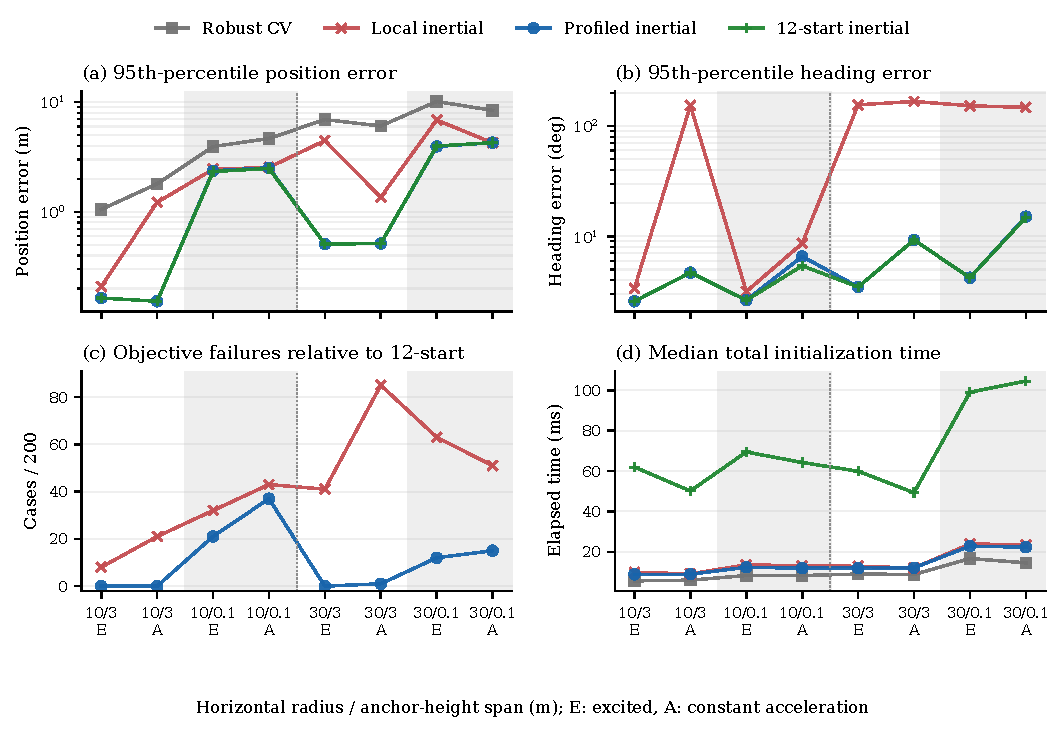
\includegraphics[width=0.98\textwidth]{geometry_stress.pdf}
 \caption{Stand-off and vertical-geometry stress test, with 200 paired seeds per cell. Profiling reduces raw-range objective misses and severe heading tails relative to one local refinement. The twelve-start reference uses the same objective, seed translation, and stopping rules. Gray regions identify the 0.1 m vertical-span cases, where height ambiguity remains. Timing is per-fit wall time under the same 20-worker desktop load, not embedded worst-case execution time.}
 \label{fig:geometry}
\end{figure*}

\subsection{Physical IMU Mismatch Separates Optimization from Accuracy}
Table~\ref{tab:imumismatch} shows that the single profiled candidate retains its objective advantage under the specified mild mismatch: it matches the twelve-start objective in all 200 cases, while the local seed misses in 57. Nevertheless, both profiling and twelve starts have a 95th-percentile position error of $1.031$ m and physical heading error of $16.90^\circ$, substantially above their ideal-input errors. The candidate improves optimization reliability; it does not remove calibration error. Before optimization, the 95th percentile of maximum sampled-displacement error is $1.90$ m at the mild level and $8.09$ m at the moderate level.

At the moderate level, profiling misses the reference objective in 31 of 200 cases and its 95th-percentile position error reaches $4.698$ m. The twelve-start reference reduces that position quantile to $4.223$ m, but has a larger heading quantile: $133.85^\circ$ versus $52.10^\circ$ for profiling. Thus a lower mis-specified raw-range objective can correspond to a worse physical heading. None of these tails supports accurate, general recovery under the moderate condition. This result strengthens the distinction between the conditional algebraic guarantee, practical optimization, and physical navigation accuracy; it also motivates explicit inertial uncertainty or bias estimation beyond the fixed-bias candidate.

\begin{table}[t]
\caption{Physical IMU calibration mismatch: 200 paired seeds per level. Misses are relative to twelve starts; $e_{p,95}$ and $e_{h,95}$ are 95th-percentile position and physical endpoint-heading errors. Levels are defined in Section~\ref{sec:imuprotocol}.}
\label{tab:imumismatch}
\centering
\setlength{\tabcolsep}{3.5pt}
\begin{tabular}{llrrr}
\toprule
Level&Method&Misses&$e_{p,95}$ (m)&$e_{h,95}$ ($^\circ$)\\
\midrule
Ideal&Local&53&4.221&161.26\\
&Profile&0&0.546&3.58\\
&Twelve starts&0&0.546&3.58\\
\midrule
Mild&Local&57&4.254&161.05\\
&Profile&0&1.031&16.90\\
&Twelve starts&0&1.031&16.90\\
\midrule
Moderate&Local&65&5.902&156.75\\
&Profile&31&4.698&52.10\\
&Twelve starts&0&4.223&133.85\\
\bottomrule
\end{tabular}
\end{table}

The matched model-order ablation in Table~\ref{tab:order} clarifies the role of polynomial nuisance absorption. With ideal inertial input, $K=2$ increases position and heading tails, consistent with its additional nuisance freedom. Under moderate combined mismatch, however, it reduces the 95th-percentile position error from $4.535$ to $0.761$ m and physical heading error from $54.85^\circ$ to $12.39^\circ$ relative to $K=1$ with the same two-seed policy. This is an empirical approximation benefit under rotating attitude and combined errors, not an extension of exact polynomial invariance to arbitrary gyroscope or tilt errors. It identifies a useful model-order choice rather than a universally preferable order.

\begin{table}[t]
\caption{Matched polynomial-order ablation: 200 paired trials per level, with two translation seeds for both models. Position and physical heading errors are 95th percentiles.}
\label{tab:order}
\centering
\setlength{\tabcolsep}{5pt}
\begin{tabular}{lrrrr}
\toprule
&\multicolumn{2}{c}{$K=1$, two seeds}&\multicolumn{2}{c}{$K=2$, two seeds}\\
\cmidrule(lr){2-3}\cmidrule(lr){4-5}
Level&Position (m)&Heading ($^\circ$)&Position (m)&Heading ($^\circ$)\\
\midrule
Ideal&0.546&3.58&0.732&4.75\\
Mild&1.031&16.90&0.731&5.52\\
Moderate&4.535&54.85&0.761&12.39\\
\bottomrule
\end{tabular}
\end{table}

\subsection{Bias Elimination Changes Both Accuracy and the Meaning of Information}
Figure~\ref{fig:bias} isolates the effect of the assumed bias model. At a component bias standard deviation of $0.3\,\mathrm{m/s^2}$ in excited motion, fixed-bias estimation has a median heading error of approximately $\BiasFixedYaw^\circ$ and position error of $\BiasFixedPosition$ m. Free-bias polynomial estimation reduces these to approximately $\BiasFreeYaw^\circ$ and $\BiasFreePosition$ m in this controlled constant-attitude experiment. This is a substantial conditional effect: the excitation allows the nonquadratic inertial signal to be separated from a quadratic bias contribution.

Under constant acceleration, the result is qualitatively different. After free-bias elimination, median yaw information is approximately $3.2\times10^{-26}$ and none of 1,000 cases satisfies the acceptance criterion. The corresponding median position error is $0.067$ m because a polynomial trajectory is still recoverable. The algorithm is recognizing an ambiguity, not recovering heading. At $0.3\,\mathrm{m/s^2}$ bias scale, the fixed-bias test accepts 992 of 1,000 cases, with 554 accepted but inaccurate headings. This contrast is consistent with the explicit equivalent-solution construction \eqref{eq:biasambiguity}.

The two polynomial orders are model ablations with different assumptions, rather than interchangeable implementations of a complete 15-state initializer. This constant-world-bias experiment isolates accelerometer-bias contamination; the separate physical IMU study tests specified combined calibration errors. Neither includes IMU measurement noise or an unknown UWB lever arm.

\subsection{Real-Window Candidate Reliability}\label{sec:windowresults}
Table~\ref{tab:windows} and Fig.~\ref{fig:windows} show that circle-based candidate generation also changes the achieved objective on real measurements. A single profiled seed reduces total misses from 87 to 40 out of 528 configurations while reducing the total function evaluations from 36,157 to 32,632, including the common CV fit. The paired comparison contains 58 cases where profiling alone reaches the best observed objective and 11 where the local seed alone does; both miss in 29. These are paired computational outcomes, with configurations correlated by recording and physical window.

Refining additional circle candidates improves reliability: Profile-2 misses 28 configurations, and Profile-all misses 11. The stronger four-uniform-start baseline misses 12 with fewer total function evaluations than Profile-all. Their advantage depends on geometry: Uniform-4 is better with all eight anchors (one versus five misses), whereas Profile-all is better with the lower four (six versus eleven). Uniform-12 has no objective misses at this tolerance, at a much larger evaluation count. The circle candidates therefore offer a useful single-refinement improvement and an alternative seed allocation under reduced vertical geometry; they do not uniformly dominate every multi-start budget. The best observed objective remains a numerical reference, and a smaller real-data range residual is not a substitute for unavailable heading truth.

Increasing the objective tolerance from $10^{-4}$ to $10^{-3}$ leaves all six miss counts unchanged. At $10^{-2}$, Local, Profile-1, Profile-2, Profile-all, Uniform-4, and Uniform-12 miss 83, 36, 24, 8, 11, and 0 configurations, respectively. The principal comparison is therefore not a consequence of round-off-level objective differences.

\begin{table}[t]
\caption{Matched real-window optimization. Each geometry contains 264 configurations; misses use the joint best observed objective and the tolerance in Section~\ref{sec:realwindowprotocol}. Evaluation totals include the CV seed. Time is the median/95th percentile on a separate sequential timing subset.}
\label{tab:windows}
\centering
\setlength{\tabcolsep}{3.1pt}
\begin{tabular}{lrrrr}
\toprule
&\multicolumn{2}{c}{Misses}&Function&Time\\
\cmidrule(lr){2-3}
Method&All 8&Low 4&evaluations&(ms)\\
\midrule
Local&31&56&36,157&15.54/63.35\\
Profile-1&15&25&32,632&13.28/65.58\\
Profile-2&9&19&47,466&17.79/85.83\\
Profile-all&5&6&93,690&37.01/158.54\\
Uniform-4&1&11&85,229&33.44/139.58\\
Uniform-12&0&0&216,893&83.08/364.02\\
\bottomrule
\end{tabular}
\end{table}

\begin{figure*}[t]
 \centering
 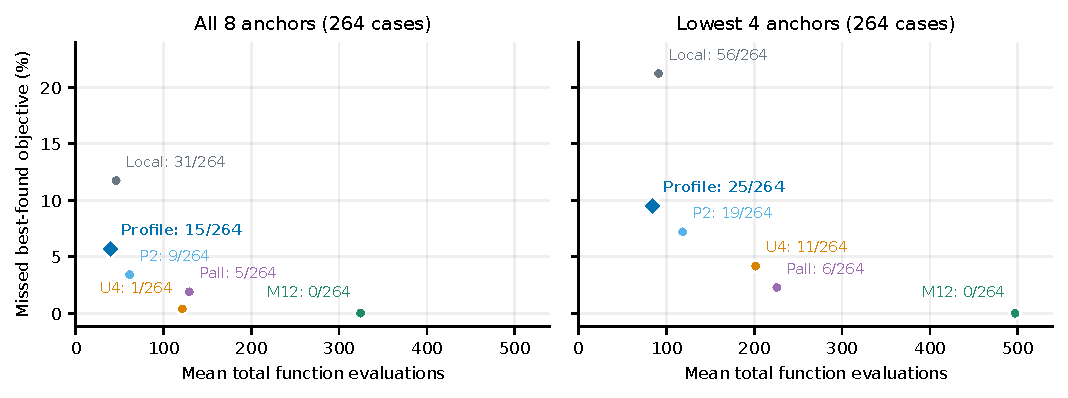
\includegraphics[width=0.98\textwidth]{window_solver_tradeoff.pdf}
 \caption{Real-window objective quality and computational work, including both solves of the common CV seed. P2 and Pall denote Profile-2 and Profile-all; U4 and M12 denote Uniform-4 and Uniform-12. The profiled single seed improves upon one local refinement in both anchor subsets, while the relative advantage of multiple circular and uniform seeds depends on geometry. Cases are correlated configurations from the same six development logs.}
 \label{fig:windows}
\end{figure*}

\subsection{Complete Real-Data Replays Have Similar Terminal Accuracy}
Table~\ref{tab:real} shows that robust constant-velocity, local inertial, twelve-start, and profiled initialization all achieve five stable successes out of six during continuous ranging. Their common-interval median RMSE is approximately $0.285$ m. The square recording is the shared stable-success failure; its terminal five-second RMSE is approximately $0.39$ m, illustrating that a failure of the sustained $0.5$ m criterion need not mean a large final RMS error.

The maximum available-output error is approximately $1.50$ m for the fixed-window methods, compared with $16.27$ m for historical lifted capture, but the former wait two seconds before publishing an initial state whereas lifted capture publishes throughout acquisition. Thus the difference combines acquisition error and availability. The near-identical terminal performance of robust CV and the inertial initializers shows that eventual tracker accuracy need not reveal differences in window-level optimization reliability.

Enabling the historical capture's gate from the first measurement does not reliably solve acquisition: it reduces stable success and produces a finite multi-kilometer failure in one log. A range-rejection policy designed for tracking can reject the evidence needed to recover a wrong state. Conversely, disabling rejection permits large early updates. These observations justify a separate acquisition stage, but they do not favor one particular lift or information threshold by themselves.

A separate first-second diagnostic deliberately initializes position from truth to isolate the early-excursion mechanism; it is not part of the cold-start evaluation. In the random log with an 8 m position standard deviation, the second update has a truth-referenced corrected-range error of $7.883$ m and normalized innovation squared of $18.441$. Warm-up nevertheless accepts it, producing a $34.117$ m position jump with only a $0.0091$ rad attitude injection. Hard gating from the first update limits the maximum error in that diagnostic to $0.324$ m, whereas Huber weighting alone still permits a $33.972$ m excursion. Conversely, a narrow prior with a 9 m initial position error remains badly displaced when early ranges are rejected. The first large excursion is therefore supported as an interaction of a bad range, sequentially evolving uncertainty, and disabled rejection; it cannot be attributed to a large-angle group injection at that event.

\subsection{Ranging-Outage Recovery Remains Unresolved}
During the ten-second outage, inertial propagation causes substantial drift. All four fixed-window methods recover stable terminal behavior on five of six logs, but their complete available-output excursions remain large. The profiled method reaches a maximum of approximately $27.72$ m and a common-interval median RMSE of $2.16$ m, while historical lifted capture yields about $17.65$ m and $1.39$ m, respectively. The new candidate consequently does not improve the overall outage transient in this experiment.

Waiting for the provisional information criterion is not uniformly beneficial. The adaptive method obtains only four continuous-ranging stable successes and leaves one recording entirely uninitialized. In outage tests it later acquires that record, giving five stable successes, but its reduced availability and longer wait remain part of the outcome. Reporting only the median error of available samples would conceal this cost. A complete supervisor must decide which state components can be used during weak heading observability and how to maintain bounded output errors while gathering more evidence; the present all-or-nothing threshold does not resolve that problem.

\subsection{Rotating-IMU Bias-Model Ablation}
An additional 60 replays test a ten-variable $p_T,v_T,\psi,\delta b_a$ optimizer using the physically correct $B_a(t)$ in \eqref{eq:fullbias}, a $0.10\,\mathrm{m/s^2}$ Gaussian bias prior, and the same invariant tracker. Data-only yaw information excludes that prior. Fixed 2, 4, and 8 s windows and a twelve-start 2 s variant again achieve five successes out of six in each regime. The 2/4/8 s common-interval median RMSEs are $0.285/0.284/0.289$ m with continuous ranging but $2.332/4.349/11.550$ m with an outage, compared with $2.164$ m for the fixed-bias local initializer. The 8 s variant reaches $93.02$ m during the prolonged propagated-output interval. An information-gated variant again leaves one normal log uninitialized. These tests do not show a real-data recovery benefit from the more complete bias model; the favorable controlled bias result is insufficient by itself.

\subsection{Computation and Reproducibility}
Experiments run on a Windows desktop with an Intel Core Ultra 7 265KF processor using process-level parallelism and one BLAS thread per worker. The implementation uses the project's Python environment, NumPy, SciPy, and the existing invariant tracker. In the 30 m, 3 m-height excited stress cell, median solve times are 12.83, 11.88, and 59.90 ms for local, profiled, and twelve-start refinement under the same 20-worker load. Profiling thus attains the reference objective at approximately one fifth of the median measured time in that cell. The original near-field excited trials give 6.006, 5.854, and 37.613 ms, respectively. These timings are neither target-hardware latency guarantees nor worst-case execution times. Profiling uses one circular solve and one refinement after a common robust translation seed; twelve-start performs twelve refinements.

The real-window timing subset uses twelve configurations selected before timing, ten repeats, and six methods, giving 720 sequential fits. No other Python process was active at its start. Timing includes the CV seed, all candidate refinements, and final curvature construction. Profile-1 has a 14.5\% lower median time than local initialization but a slightly higher 95th percentile, so its latency is not uniformly lower (Table~\ref{tab:windows}). Function-evaluation counts exclude linear-algebra operations such as the singular value decomposition and quartic solve; measured wall time includes them. Neither timing nor lower range residual establishes an equivalent improvement in real position error under model mismatch.

Full real trajectories, initialization attempts, accepted and rejected handoffs, range-gap triggers, metrics, configuration, and source fingerprints are retained. All 96 main and 60 bias-extension trajectories were independently rescored, with a maximum metric discrepancy of $3.6\times10^{-15}$. All geometry summary cells were checked against saved per-fit records, and 20 randomly selected cases (80 fits) were independently rerun with identical numerical results. For the physical IMU study, 20 predetermined cases (180 fits) were rerun in fresh processes and all nine summary cells independently recomputed, with numerical discrepancies below $2.3\times10^{-13}$. All 1,800 outputs were finite, and ideal-input displacement consistency was below $1.5\times10^{-13}$ m. Each polynomial order was separately audited by 60 fresh-process reruns, agreeing within $9.1\times10^{-13}$; all 1,200 ablation outputs were finite and converged. Random seeds pair synthetic conditions. Method-level or sample-level replication is not independent data collection: real uncertainty should ultimately be assessed by recording session or environment. No significance claim is made from six previously exposed, same-date evaluation logs.

Supplementary figures are distributed with the manuscript. The file \emph{trajectories.pdf} shows complete error histories during continuous ranging and the outage, including missing startup outputs and propagated recapture intervals. Other supplied plots illustrate the information geometry and additional baseline comparisons.

\section{Limitations and Research Implications}\label{sec:limits}
The exact reduction and noiseless recovery condition apply to the specified short-window model. They do not prove global tracker convergence, global raw-range optimality, or covariance consistency. Relative to polynomial-localization\cite{pacholska2020} and algebraic-pose\cite{trawny2010} methods, the specialization studied here keeps the inertial displacement as a supplied shape while profiling velocity and bias-related translation directions. Its value depends on retaining sufficient excitation after that elimination.

The main empirical gap is external validation. Same-date development logs provide position but not complete attitude or bias truth, preventing full-state NEES and heading-error assessment. The physical IMU experiment adds combined calibration mismatch but still omits IMU measurement white noise, time-varying bias, and uncertain timing. Fresh dates, anchor geometries, and independent attitude measurements are needed to establish the bias benefit beyond controlled simulation.

The constant-world-bias extension also needs care. For time-varying $Q(t)$, write the inertial displacement sensitivity as
\begin{equation}
 d_{\mathrm{true}}(t)=d_{\mathrm{nom}}(t)-B_a(t)\,\delta b_a,
 \label{eq:fullbias}
\end{equation}
where $B_a$ is the reanchored double integral of $Q$. Replacing $B_a\delta b_a$ by an unrestricted quadratic translation is then an approximation. A complete estimator should optimize the physically correct sensitivity, distinguish bias priors from data information, and propagate the resulting joint uncertainty. Static calibration alone cannot establish that the required biases are known.

Robust CV initialization matches real-data stable success, the adaptive criterion reduces availability, and outage transients remain worse than the historical lifted control. These outcomes distinguish the demonstrated initialization benefit from complete navigation performance. A practical acquisition supervisor must use the candidate without confusing conditional yaw information with full-state confidence. Evaluation on independent data and against recent moving-horizon methods\cite{pfeiffer2025}, with explicit availability and uncertainty coverage, remains necessary.

\section{Conclusion}
\balance
We derived a yaw-profile initializer for asynchronous TWR and an inertial displacement, reducing linear nuisance elimination and a circle constraint to quartic candidate enumeration. A sufficient noise-free recovery condition, polynomial-contamination invariance, and a bounded-rotation approximation identify the model's guarantees and limits. In paired far-field trials with useful vertical anchor geometry, profiling substantially reduces local-refinement failures and approaches twelve-start accuracy at lower measured computational cost. The real-window study also shows fewer raw-objective misses for a single profiled candidate, while comparisons with four and twelve uniform seeds expose the cost of additional robustness. Quadratic nuisance modeling improves accuracy under both controlled constant bias and the tested combined IMU mismatch, with an ideal-input accuracy cost exposed by the matched model-order comparison. Constant acceleration remains ambiguous when bias is unrestricted. Complete real-log replays retain similar terminal success across strong initializers and expose unresolved outage and availability issues. The resulting contribution is a more reliable initialization primitive with explicit bias assumptions, suitable for further evaluation within range--inertial acquisition systems.

\bibliographystyle{IEEEtran}
\bibliography{recovery_bootstrap_refs}
\end{document}
